\documentclass[twoside]{book}

% Packages required by doxygen
\usepackage{fixltx2e}
\usepackage{calc}
\usepackage{doxygen}
\usepackage[export]{adjustbox} % also loads graphicx
\usepackage{graphicx}
\usepackage[utf8]{inputenc}
\usepackage{makeidx}
\usepackage{multicol}
\usepackage{multirow}
\PassOptionsToPackage{warn}{textcomp}
\usepackage{textcomp}
\usepackage[nointegrals]{wasysym}
\usepackage[table]{xcolor}

% Font selection
\usepackage[T1]{fontenc}
\usepackage[scaled=.90]{helvet}
\usepackage{courier}
\usepackage{amssymb}
\usepackage{sectsty}
\renewcommand{\familydefault}{\sfdefault}
\allsectionsfont{%
  \fontseries{bc}\selectfont%
  \color{darkgray}%
}
\renewcommand{\DoxyLabelFont}{%
  \fontseries{bc}\selectfont%
  \color{darkgray}%
}
\newcommand{\+}{\discretionary{\mbox{\scriptsize$\hookleftarrow$}}{}{}}

% Page & text layout
\usepackage{geometry}
\geometry{%
  a4paper,%
  top=2.5cm,%
  bottom=2.5cm,%
  left=2.5cm,%
  right=2.5cm%
}
\tolerance=750
\hfuzz=15pt
\hbadness=750
\setlength{\emergencystretch}{15pt}
\setlength{\parindent}{0cm}
\setlength{\parskip}{3ex plus 2ex minus 2ex}
\makeatletter
\renewcommand{\paragraph}{%
  \@startsection{paragraph}{4}{0ex}{-1.0ex}{1.0ex}{%
    \normalfont\normalsize\bfseries\SS@parafont%
  }%
}
\renewcommand{\subparagraph}{%
  \@startsection{subparagraph}{5}{0ex}{-1.0ex}{1.0ex}{%
    \normalfont\normalsize\bfseries\SS@subparafont%
  }%
}
\makeatother

% Headers & footers
\usepackage{fancyhdr}
\pagestyle{fancyplain}
\fancyhead[LE]{\fancyplain{}{\bfseries\thepage}}
\fancyhead[CE]{\fancyplain{}{}}
\fancyhead[RE]{\fancyplain{}{\bfseries\leftmark}}
\fancyhead[LO]{\fancyplain{}{\bfseries\rightmark}}
\fancyhead[CO]{\fancyplain{}{}}
\fancyhead[RO]{\fancyplain{}{\bfseries\thepage}}
\fancyfoot[LE]{\fancyplain{}{}}
\fancyfoot[CE]{\fancyplain{}{}}
\fancyfoot[RE]{\fancyplain{}{\bfseries\scriptsize Generated by Doxygen }}
\fancyfoot[LO]{\fancyplain{}{\bfseries\scriptsize Generated by Doxygen }}
\fancyfoot[CO]{\fancyplain{}{}}
\fancyfoot[RO]{\fancyplain{}{}}
\renewcommand{\footrulewidth}{0.4pt}
\renewcommand{\chaptermark}[1]{%
  \markboth{#1}{}%
}
\renewcommand{\sectionmark}[1]{%
  \markright{\thesection\ #1}%
}

% Indices & bibliography
\usepackage{natbib}
\usepackage[titles]{tocloft}
\setcounter{tocdepth}{3}
\setcounter{secnumdepth}{5}
\makeindex

% Hyperlinks (required, but should be loaded last)
\usepackage{ifpdf}
\ifpdf
  \usepackage[pdftex,pagebackref=true]{hyperref}
\else
  \usepackage[ps2pdf,pagebackref=true]{hyperref}
\fi
\hypersetup{%
  colorlinks=true,%
  linkcolor=blue,%
  citecolor=blue,%
  unicode%
}

% Custom commands
\newcommand{\clearemptydoublepage}{%
  \newpage{\pagestyle{empty}\cleardoublepage}%
}

\usepackage{caption}
\captionsetup{labelsep=space,justification=centering,font={bf},singlelinecheck=off,skip=4pt,position=top}

%===== C O N T E N T S =====

\begin{document}

% Titlepage & ToC
\hypersetup{pageanchor=false,
             bookmarksnumbered=true,
             pdfencoding=unicode
            }
\pagenumbering{alph}
\begin{titlepage}
\vspace*{7cm}
\begin{center}%
{\Large F\+T\+C\+Scout }\\
\vspace*{1cm}
{\large Generated by Doxygen 1.8.12}\\
\end{center}
\end{titlepage}
\clearemptydoublepage
\pagenumbering{roman}
\tableofcontents
\clearemptydoublepage
\pagenumbering{arabic}
\hypersetup{pageanchor=true}

%--- Begin generated contents ---
\chapter{Hierarchical Index}
\section{Class Hierarchy}
This inheritance list is sorted roughly, but not completely, alphabetically\+:\begin{DoxyCompactList}
\item Q\+Graphics\+Scene\begin{DoxyCompactList}
\item \contentsline{section}{Draw\+Path}{\pageref{class_draw_path}}{}
\end{DoxyCompactList}
\item Q\+Main\+Window\begin{DoxyCompactList}
\item \contentsline{section}{Main\+Window}{\pageref{class_main_window}}{}
\end{DoxyCompactList}
\item \contentsline{section}{Team}{\pageref{class_team}}{}
\end{DoxyCompactList}

\chapter{Class Index}
\section{Class List}
Here are the classes, structs, unions and interfaces with brief descriptions\+:\begin{DoxyCompactList}
\item\contentsline{section}{\hyperlink{class_draw_path}{Draw\+Path} }{\pageref{class_draw_path}}{}
\item\contentsline{section}{\hyperlink{class_main_window}{Main\+Window} \\*The \hyperlink{class_main_window}{Main\+Window} class }{\pageref{class_main_window}}{}
\item\contentsline{section}{\hyperlink{class_team}{Team} }{\pageref{class_team}}{}
\end{DoxyCompactList}

\chapter{Class Documentation}
\hypertarget{class_draw_path}{}\section{Draw\+Path Class Reference}
\label{class_draw_path}\index{Draw\+Path@{Draw\+Path}}
Inheritance diagram for Draw\+Path\+:\begin{figure}[H]
\begin{center}
\leavevmode
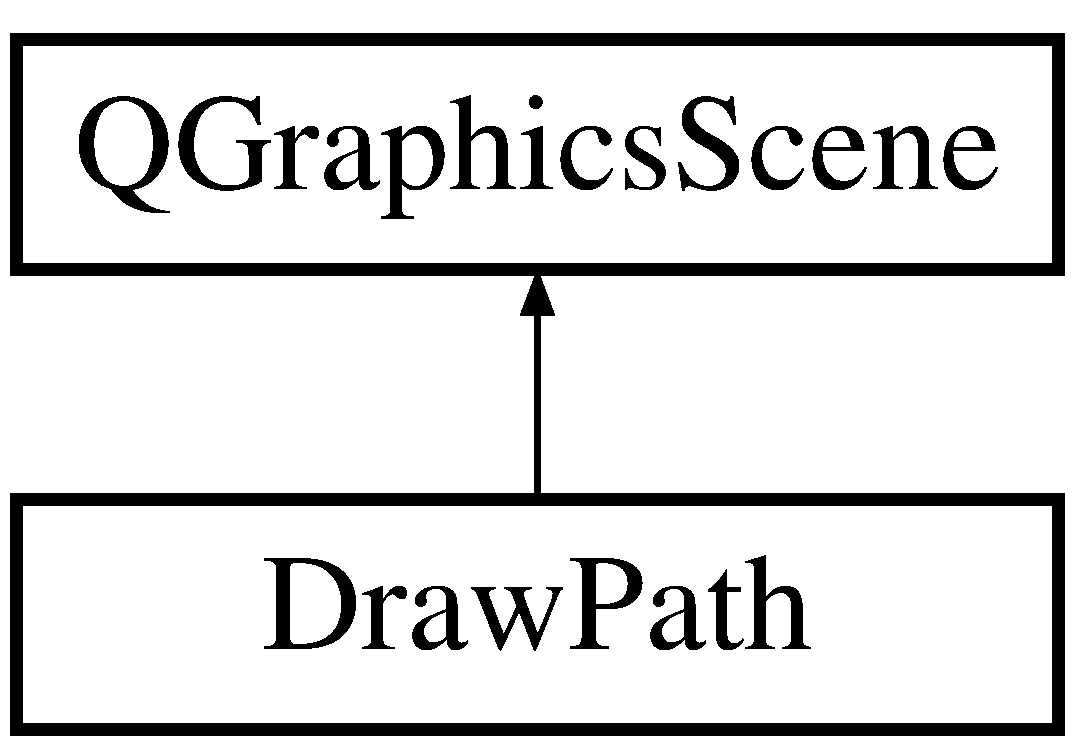
\includegraphics[height=2.000000cm]{class_draw_path}
\end{center}
\end{figure}
\subsection*{Signals}
\begin{DoxyCompactItemize}
\item 
\hypertarget{class_draw_path_ae03f0fbd38de93d428303e576d6350fc}{}\label{class_draw_path_ae03f0fbd38de93d428303e576d6350fc} 
void {\bfseries user\+Has\+Drawn} ()
\end{DoxyCompactItemize}
\subsection*{Public Member Functions}
\begin{DoxyCompactItemize}
\item 
\hypertarget{class_draw_path_aea210b1571af3051097fd3724b3de42c}{}\label{class_draw_path_aea210b1571af3051097fd3724b3de42c} 
{\bfseries Draw\+Path} (Q\+Object $\ast$parent=0)
\item 
\hypertarget{class_draw_path_a81d8d873f247eb29008dfbe4110b56ac}{}\label{class_draw_path_a81d8d873f247eb29008dfbe4110b56ac} 
void {\bfseries draw\+Field} ()
\item 
\hypertarget{class_draw_path_a73baf263dfdf3b1cc76b973547a94712}{}\label{class_draw_path_a73baf263dfdf3b1cc76b973547a94712} 
void {\bfseries print\+Path} ()
\item 
\hypertarget{class_draw_path_a51daca7fb10e584cea8040dc1ca7bb6e}{}\label{class_draw_path_a51daca7fb10e584cea8040dc1ca7bb6e} 
vector$<$ Q\+PointF $>$ {\bfseries get\+Path} ()
\item 
\hypertarget{class_draw_path_af28189ce534f4ba3dbbce2b601746d69}{}\label{class_draw_path_af28189ce534f4ba3dbbce2b601746d69} 
void {\bfseries draw\+Path} (vector$<$ Q\+PointF $>$ path)
\end{DoxyCompactItemize}
\subsection*{Public Attributes}
\begin{DoxyCompactItemize}
\item 
\hypertarget{class_draw_path_aad90fa11d471d125a9c4b9cf2b3857af}{}\label{class_draw_path_aad90fa11d471d125a9c4b9cf2b3857af} 
bool {\bfseries has\+Drawn}
\item 
\hypertarget{class_draw_path_a64bfe2eeb358500b9c27caac632d01f2}{}\label{class_draw_path_a64bfe2eeb358500b9c27caac632d01f2} 
bool {\bfseries allow\+Draw}
\end{DoxyCompactItemize}


The documentation for this class was generated from the following file\+:\begin{DoxyCompactItemize}
\item 
C\+:/\+Users/dogea/\+Desktop/\+Programming/\+Robotics/\+Scouting/\+F\+T\+C\+Scout/\+Headers/drawpath.\+h\end{DoxyCompactItemize}

\hypertarget{class_main_window}{}\section{Main\+Window Class Reference}
\label{class_main_window}\index{Main\+Window@{Main\+Window}}


The \hyperlink{class_main_window}{Main\+Window} class.  




{\ttfamily \#include $<$mainwindow.\+h$>$}

Inheritance diagram for Main\+Window\+:\begin{figure}[H]
\begin{center}
\leavevmode
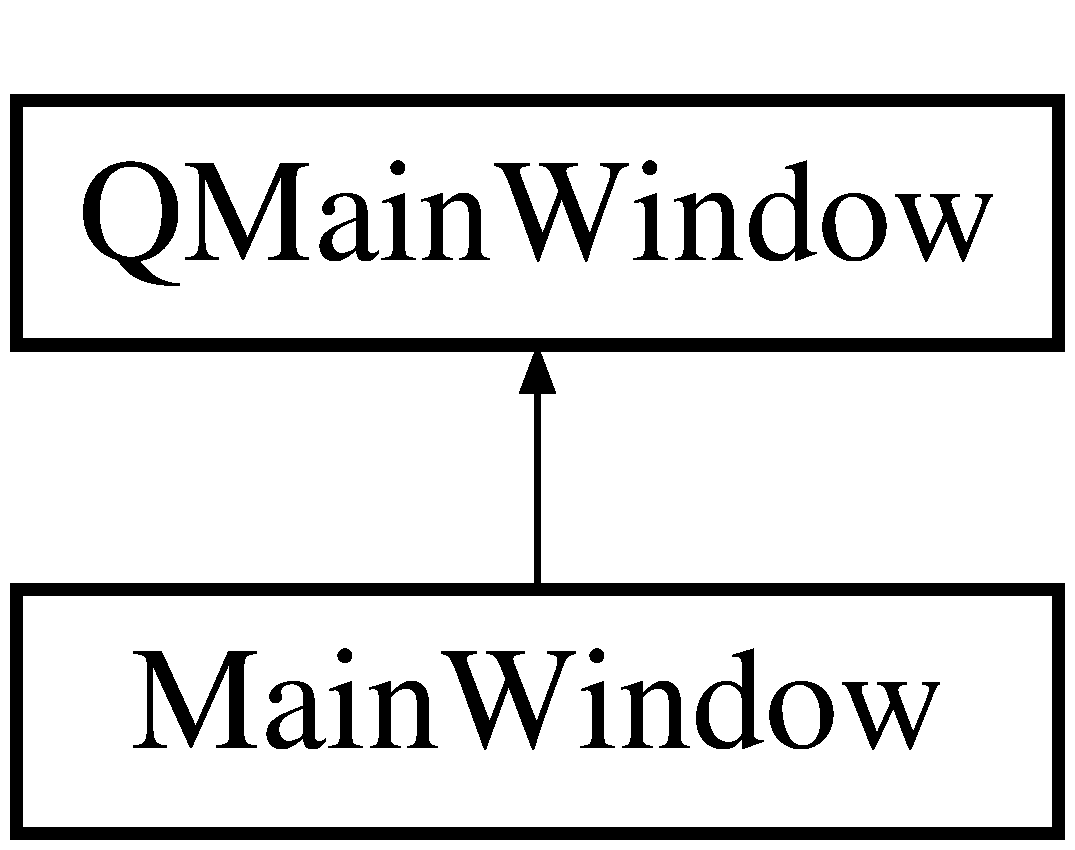
\includegraphics[height=2.000000cm]{class_main_window}
\end{center}
\end{figure}
\subsection*{Public Member Functions}
\begin{DoxyCompactItemize}
\item 
\hyperlink{class_main_window_a8b244be8b7b7db1b08de2a2acb9409db}{Main\+Window} (Q\+Widget $\ast$parent=0)
\begin{DoxyCompactList}\small\item\em Main window constructor. \end{DoxyCompactList}\end{DoxyCompactItemize}


\subsection{Detailed Description}
The \hyperlink{class_main_window}{Main\+Window} class. 

Holds elements and functions dealing with the main window 

\subsection{Constructor \& Destructor Documentation}
\hypertarget{class_main_window_a8b244be8b7b7db1b08de2a2acb9409db}{}\label{class_main_window_a8b244be8b7b7db1b08de2a2acb9409db} 
\index{Main\+Window@{Main\+Window}!Main\+Window@{Main\+Window}}
\index{Main\+Window@{Main\+Window}!Main\+Window@{Main\+Window}}
\subsubsection{\texorpdfstring{Main\+Window()}{MainWindow()}}
{\footnotesize\ttfamily Main\+Window\+::\+Main\+Window (\begin{DoxyParamCaption}\item[{Q\+Widget $\ast$}]{parent = {\ttfamily 0} }\end{DoxyParamCaption})\hspace{0.3cm}{\ttfamily [explicit]}}



Main window constructor. 


\begin{DoxyParams}{Parameters}
{\em parent} & A Q\+Widget\\
\hline
\end{DoxyParams}
Not used 

The documentation for this class was generated from the following file\+:\begin{DoxyCompactItemize}
\item 
C\+:/\+Users/dogea/\+Desktop/\+Programming/\+Robotics/\+Scouting/\+F\+T\+C\+Scout/\+Headers/mainwindow.\+h\end{DoxyCompactItemize}

\hypertarget{class_team}{}\section{Team Class Reference}
\label{class_team}\index{Team@{Team}}
\subsection*{Public Member Functions}
\begin{DoxyCompactItemize}
\item 
\hypertarget{class_team_a3119f904a89b3806829bd49bd31b0e28}{}\label{class_team_a3119f904a89b3806829bd49bd31b0e28} 
{\bfseries Team} (int team\+Number)
\item 
\hypertarget{class_team_a76485312b881e585ccfa227710e708e8}{}\label{class_team_a76485312b881e585ccfa227710e708e8} 
int {\bfseries get\+Number} ()
\item 
\hypertarget{class_team_a8de8a2cfe74dbbb12660fe1cf462182a}{}\label{class_team_a8de8a2cfe74dbbb12660fe1cf462182a} 
void {\bfseries set\+Number} (int num)
\item 
\hypertarget{class_team_ab21736a411213da36d08210e570ecbeb}{}\label{class_team_ab21736a411213da36d08210e570ecbeb} 
string {\bfseries get\+Name} ()
\item 
\hypertarget{class_team_a6b4e344f80d411949578889098b7194b}{}\label{class_team_a6b4e344f80d411949578889098b7194b} 
void {\bfseries set\+Name} (string str)
\item 
\hypertarget{class_team_a9895de1b3518a9bb7e57d636a056b75b}{}\label{class_team_a9895de1b3518a9bb7e57d636a056b75b} 
int {\bfseries get\+Place} ()
\item 
\hypertarget{class_team_aeed30ef27240a1ee2c127619031b40cf}{}\label{class_team_aeed30ef27240a1ee2c127619031b40cf} 
void {\bfseries set\+Place} (int num)
\item 
\hypertarget{class_team_aac0ef50b17408230d4435e64e0a0c0c0}{}\label{class_team_aac0ef50b17408230d4435e64e0a0c0c0} 
int {\bfseries get\+Tele\+Op\+Element} (int i)
\item 
\hypertarget{class_team_aeecb192d3474abbebfa0582d303cd7da}{}\label{class_team_aeecb192d3474abbebfa0582d303cd7da} 
void {\bfseries set\+Tele\+Op\+Element} (int i, bool num)
\item 
\hypertarget{class_team_a655dced0629f619cca497d36adcdd1eb}{}\label{class_team_a655dced0629f619cca497d36adcdd1eb} 
int {\bfseries get\+Auto\+Element} (int i)
\item 
\hypertarget{class_team_ada705e237131e8e1e57f341f3189d217}{}\label{class_team_ada705e237131e8e1e57f341f3189d217} 
void {\bfseries set\+Auto\+Element} (int i, bool num)
\item 
\hypertarget{class_team_ade87e9b263d6db2fe6182d452b6d1c86}{}\label{class_team_ade87e9b263d6db2fe6182d452b6d1c86} 
void {\bfseries add\+To\+Path\+List} (vector$<$ Q\+PointF $>$ path)
\item 
\hypertarget{class_team_a817413d08a986d587cfc3f956747d302}{}\label{class_team_a817413d08a986d587cfc3f956747d302} 
vector$<$ Q\+PointF $>$ {\bfseries get\+Single\+Path} (int i)
\item 
\hypertarget{class_team_a428e94b1b2cd8cc9ac98cc1b1a99f9bd}{}\label{class_team_a428e94b1b2cd8cc9ac98cc1b1a99f9bd} 
vector$<$ vector$<$ Q\+PointF $>$ $>$ {\bfseries get\+Paths} ()
\item 
\hypertarget{class_team_a42c7673c22080863593daf8b1634d2f4}{}\label{class_team_a42c7673c22080863593daf8b1634d2f4} 
string {\bfseries get\+Other} ()
\item 
\hypertarget{class_team_a404115b44f2a98a0771126a61d6f35d2}{}\label{class_team_a404115b44f2a98a0771126a61d6f35d2} 
void {\bfseries set\+Other} (string str)
\item 
\hypertarget{class_team_a8245bef50c20b4b5caed0525ebbfaea5}{}\label{class_team_a8245bef50c20b4b5caed0525ebbfaea5} 
void {\bfseries write\+To\+File} (string file\+Name)
\item 
\hypertarget{class_team_adc5f6d480da08975cfdb402a4ec9844c}{}\label{class_team_adc5f6d480da08975cfdb402a4ec9844c} 
int {\bfseries read\+From\+File} (string file\+Name, int target\+Read\+Number, vector$<$ \hyperlink{class_team}{Team} $>$ already\+Read)
\item 
\hypertarget{class_team_adc86367c9f0132e20df8f7d336e8eed2}{}\label{class_team_adc86367c9f0132e20df8f7d336e8eed2} 
void {\bfseries erase\+Path} (int index)
\item 
\hypertarget{class_team_a44f8d9369753d254028b4508490b687e}{}\label{class_team_a44f8d9369753d254028b4508490b687e} 
void {\bfseries erase\+All\+Paths} ()
\end{DoxyCompactItemize}
\subsection*{Static Public Attributes}
\begin{DoxyCompactItemize}
\item 
\hypertarget{class_team_abd61cb331b997f7dc6a355886de59fc7}{}\label{class_team_abd61cb331b997f7dc6a355886de59fc7} 
static const int {\bfseries T\+E\+L\+E\+O\+P\+\_\+\+N\+U\+M\+\_\+\+A\+B\+I\+L\+I\+T\+I\+ES} = 3
\item 
\hypertarget{class_team_ac9866eaa1c3385d129ea663c34587717}{}\label{class_team_ac9866eaa1c3385d129ea663c34587717} 
static const int {\bfseries A\+U\+T\+O\+\_\+\+N\+U\+M\+\_\+\+A\+B\+I\+L\+I\+T\+I\+ES} = 3
\end{DoxyCompactItemize}


The documentation for this class was generated from the following file\+:\begin{DoxyCompactItemize}
\item 
C\+:/\+Users/dogea/\+Desktop/\+Programming/\+Robotics/\+Scouting/\+F\+T\+C\+Scout/\+Headers/team.\+h\end{DoxyCompactItemize}

%--- End generated contents ---

% Index
\backmatter
\newpage
\phantomsection
\clearemptydoublepage
\addcontentsline{toc}{chapter}{Index}
\printindex

\end{document}
